\documentclass[12pt,a4paper]{article}

% ============ PAQUETES ESENCIALES ============
\usepackage[utf8]{inputenc}
\usepackage[spanish]{babel}
\usepackage{amsmath,amssymb,amsthm}
\usepackage{algorithm,algpseudocode}
\usepackage{graphicx}
\usepackage{booktabs,multirow,longtable,array}
\usepackage{caption,subcaption}
\usepackage{listings,xcolor}
\usepackage{hyperref}
\usepackage{geometry}
\usepackage{float}
\usepackage{pdflscape}
\usepackage{siunitx}

\geometry{margin=2.5cm}

% ============ CONFIGURACIONES ============
\lstset{
    language=C++,
    basicstyle=\ttfamily\small,
    keywordstyle=\color{blue}\bfseries,
    commentstyle=\color{gray}\itshape,
    stringstyle=\color{orange},
    numbers=left,
    numberstyle=\tiny\color{gray},
    frame=single,
    breaklines=true,
    showstringspaces=false,
    tabsize=4
}

\hypersetup{
    colorlinks=true,
    linkcolor=blue,
    citecolor=blue,
    urlcolor=blue,
    pdftitle={PCA e Identificacion de Ancestra Genetica},
    pdfauthor={Autor}
}

% ============ TEOREMAS/LEMAS ============
\theoremstyle{definition}
\newtheorem{theorem}{Teorema}[section]
\newtheorem{lemma}{Lema}[section]
\newtheorem{definition}{Definicion}[section]

% ============ COMANDOS PERSONALIZADOS ============
\newcommand{\normF}[1]{\|#1\|_F}
\newcommand{\R}{\mathbb{R}}

% ============ DOCUMENTO ============
\begin{document}

% ---------- PORTADA ----------
\begin{titlepage}
    \centering
    \vspace*{2cm}
    {\Huge\bfseries An\'{a}lisis de Componentes Principales (PCA)\\[0.3cm] e Identificaci\'{o}n de Ancestr\'{i}a Gen\'{e}tica\par}
    \vspace{1.5cm}
    {\Large Informe T\'{e}cnico de Implementaci\'{o}n y Resultados\par}
    \vspace{2cm}
    {\Large Autor: Gregory Uzcategui / CI: 27.376.191 \par}
    \vspace{2cm}
    {\large
    \textbf{Stack tecnol\'{o}gico:} C++17 (Eigen 3.4, fast-cpp-csv-parser), CMake, Python 3 (matplotlib, numpy, pandas)\\[0.5cm]
    \textbf{Algoritmo:} Eigen::BDCSVD (Divide-and-Conquer)\\[0.5cm]
    \textbf{Dataset:} 30 individuos diploides $\times$ 100 SNPs, codificaci\'{o}n $\{0,1,2\}$
    \par}
    \vfill
    {\large \today\par}
\end{titlepage}

% ---------- RESUMEN ----------
\begin{abstract}
\noindent
Este informe documenta la implementaci\'{o}n de un pipeline computacional para el an\'{a}lisis de estructura poblacional mediante Componentes Principales (PCA) aplicado a datos gen\'{e}ticos de SNPs. Se proces\'{o} una matriz de genotipos $G \in \R^{100 \times 30}$ (100 SNPs, 30 individuos diploides), codificada en $\{0,1,2\}$. El flujo incluye: estimaci\'{o}n de frecuencias al\'{e}licas, filtrado de SNPs constantes, normalizaci\'{o}n de Patterson (Wright-Fisher), descomposici\'{o}n en valores singulares (SVD) y proyecci\'{o}n al espacio de componentes principales $PC = U\Sigma$. 
\end{abstract}

\tableofcontents
\newpage

% ---------- 1. INTRODUCCION ----------
\section{Introducci\'{o}n}\label{sec:intro}

El estudio de la variabilidad gen\'{e}tica humana se fundamenta en la identificaci\'{o}n de polimorfismos de nucle\'{o}tido \'unico (SNPs), que constituyen los cambios m\'{i}nimos en la secuencia del ADN. Dada la alta dimensionalidad de estos datos ---donde el n\'{u}mero de sitios gen\'{e}ticos suele superar por \'ordenes de magnitud al n\'{u}mero de individuos---, el An\'{a}lisis de Componentes Principales (PCA) se ha consolidado como la herramienta est\'{a}ndar para visualizar la estructura poblacional y detectar procesos de mezcla migratoria (admixture) \cite{patterson2006}.

Este proyecto implementa el flujo de c\'{a}lculo num\'{e}rico completo para transformar datos crudos de genotipos en un mapa de ancestr\'{i}a, utilizando la Descomposici\'{o}n en Valores Singulares (SVD) como m\'{e}todo num\'{e}rico central. La implementaci\'{o}n se realiza en C++17 con la biblioteca Eigen 3.4 para \'algebra lineal,  mientras que la visualizaci\'{o}n se gener\'{o} con Python, siguiendo una metodolog\'{i}a de especificaci\'{o}n de software (SSD) que garantiza trazabilidad entre dise\~{n}o, implementaci\'{o}n y validaci\'{o}n.

\subsection{Objetivos}
\begin{itemize}
    \item Implementar el pipeline completo de PCA gen\'{e}tico en C++17 con precisi\'{o}n de doble precisi\'{o}n.
    \item Aplicar la normalizaci\'{o}n de Patterson para garantizar contribuci\'{o}n equitativa de cada SNP.
    \item Calcular la SVD mediante \texttt{Eigen::BDCSVD} y proyectar los individuos al espacio PC1 vs PC2.
    \item Identificar visualmente clusters poblacionales y detectar individuos de mezcla (admixture).
    \item Documentar la arquitectura modular bajo metodolog\'{i}a SSD con trazabilidad especificaci\'{o}n--implementaci\'{o}n.
\end{itemize}

% ---------- 2. MARCO TEORICO ----------
\section{Marco Te\'{o}rico}\label{sec:teoria}

\subsection{Codificaci\'{o}n Genot\'{i}pica}

Los seres humanos son organismos diploides, poseyendo dos copias de cada cromosoma. Para cada posici\'{o}n evaluada (SNP), se define el alelo $A$ como la variante de referencia y el alelo $a$ como la variante mutada. La matriz de genotipos $G \in \R^{n \times m}$ se codifica como:

\begin{table}[H]
\centering
\caption{Codificaci\'{o}n genot\'{i}pica.}
\label{tab:codificacion}
\begin{tabular}{@{}cll@{}}
\toprule
\textbf{Valor} & \textbf{Genotipo} & \textbf{Significado} \\ \midrule
0 & $AA$ & Homocigoto referencia (0 copias del alelo variante) \\
1 & $Aa$ & Heterocigoto (1 copia del alelo variante) \\
2 & $aa$ & Homocigoto variante (2 copias del alelo variante) \\ \bottomrule
\end{tabular}
\end{table}

\subsection{Frecuencia del Alelo Variante}

Para cada SNP $j$ (columna de $G$), la frecuencia del alelo variante $p_j$ se estima como:
\begin{equation}\label{eq:freq}
p_j = \frac{\sum_{i=1}^{n} G_{i,j}}{2n}
\end{equation}
donde $n = 30$ es el n\'{u}mero de individuos y el denominador $2n$ refleja la condici\'{o}n diploide.

Los SNPs constantes ($p_j = 0$ o $p_j = 1$) se descartan para evitar singularidades matem\'{a}ticas en la normalizaci\'{o}n, dado que no aportan informaci\'{o}n para diferenciar poblaciones.

\subsection{Normalizaci\'{o}n de Patterson (Wright-Fisher)}

Para que cada sitio gen\'{e}tico contribuya equitativamente a la varianza, se aplica la transformaci\'{o}n:
\begin{equation}\label{eq:patterson}
\tilde{G}_{i,j} = \frac{G_{i,j} - 2p_j}{\sqrt{2p_j(1-p_j)}}
\end{equation}

El numerador $G_{i,j} - 2p_j$ representa la desviaci\'{o}n del genotipo respecto al promedio poblacional bajo equilibrio Hardy-Weinberg, mientras que el denominador $\sqrt{2p_j(1-p_j)}$ corresponde a la desviaci\'{o}n est\'{a}ndar esperada bajo deriva gen\'{e}tica neutra (modelo Wright-Fisher). El resultado es un \emph{z-score gen\'{e}tico} donde cada SNP tiene media $\approx 0$ y varianza $\approx 1$.

\subsection{Descomposici\'{o}n en Valores Singulares (SVD)}

\begin{definition}[Descomposici\'{o}n SVD]
La descomposici\'{o}n en valores singulares de la matriz normalizada transpuesta $\tilde{G}^T \in \R^{n \times m'}$ es:
\begin{equation}\label{eq:svd}
\tilde{G}^T = U \Sigma V^T
\end{equation}
donde $U \in \R^{n \times n}$ y $V \in \R^{m' \times m'}$ son matrices ortogonales, y $\Sigma \in \R^{n \times m'}$ es una matriz diagonal con valores singulares $\sigma_1 \geq \sigma_2 \geq \dots \geq \sigma_r > 0$, siendo $r = \min(n, m')$.
\end{definition}

Las coordenadas de los individuos en el espacio de componentes principales se obtienen mediante:
\begin{equation}\label{eq:pc}
PC = U \Sigma
\end{equation}

La varianza explicada por el $i$-\'{e}simo componente es:
\begin{equation}\label{eq:varianza}
\text{Varianza}_i = \frac{\sigma_i^2}{\sum_{j=1}^{r} \sigma_j^2} \times 100\%
\end{equation}

\subsection{Perspectiva de Sistemas Complejos}

La matriz $K = \frac{1}{m'}\tilde{G}\tilde{G}^T$ es an\'{a}loga a una matriz de correlaci\'{o}n o parentesco. En f\'{i}sica estad\'{i}stica, los autovectores de $K$ representan los modos de variaci\'{o}n dominantes del sistema. Los valores singulares $\sigma_i$ indican cu\'{a}nta ``energ\'{i}a'' (varianza gen\'{e}tica) captura cada modo. El PCA permite separar la se\~{n}al biol\'{o}gica (estructura poblacional) del ruido estoc\'{a}stico (deriva gen\'{e}tica neutra).

% ---------- 3. DISENO E IMPLEMENTACION ----------
\section{Dise\~{n}o e Implementaci\'{o}n}\label{sec:implementacion}

\subsection{Arquitectura del Sistema}

El proyecto sigue una arquitectura modular en C++17, separando responsabilidades en 5 m\'{o}dulos principales (Tabla~\ref{tab:modulos}).

\begin{table}[H]
\centering
\caption{M\'{o}dulos del sistema y sus responsabilidades.}
\label{tab:modulos}
\begin{tabular}{@{}lp{6cm}l@{}}
\toprule
\textbf{M\'{o}dulo} & \textbf{Responsabilidad} & \textbf{Ficheros} \\
\midrule
\texttt{cargador\_csv} & Lectura de \texttt{datos\_genotipo.csv}, validaci\'{o}n de valores $\{0,1,2\}$ & \texttt{.hpp / .cpp} \\
\texttt{procesador\_pca} & C\'{a}lculo de frecuencias $p_j$, filtrado de SNPs constantes, normalizaci\'{o}n Patterson & \texttt{.hpp / .cpp} \\
\texttt{svd\_calculador} & Descomposici\'{o}n SVD (BDCSVD) y proyecci\'{o}n $PC = U\Sigma$ & \texttt{.hpp / .cpp} \\
\texttt{exportador} & Escritura de \texttt{resultado\_pca.csv} y \texttt{varianza.csv} & \texttt{.hpp / .cpp} \\
\texttt{main} & Orquestaci\'{o}n del pipeline y logging & \texttt{main.cpp} \\
\bottomrule
\end{tabular}
\end{table}

\subsection{Stack Tecnol\'{o}gico}

\begin{table}[H]
\centering
\caption{Stack tecnol\'{o}gico del proyecto.}
\label{tab:stack}
\begin{tabular}{@{}llll@{}}
\toprule
\textbf{Capa} & \textbf{Tecnolog\'{i}a} & \textbf{Versi\'{o}n} & \textbf{Prop\'{o}sito} \\ \midrule
C\'{a}lculo num\'{e}rico & C++17 & ISO/IEC 14882:2017 & N\'{u}cleo del pipeline \\
\'{A}lgebra lineal & Eigen & 3.4+ & Matrices densas, BDCSVD \\
Parser CSV & fast-cpp-csv-parser & 1.0 (header-only) & Lectura de datos \\
Build system & CMake & 3.16+ & Generaci\'{o}n de targets \\
Visualizaci\'{o}n & Python + matplotlib & 3.10+ / 3.7+ & Scatter plot PC1 vs PC2 \\ \bottomrule
\end{tabular}
\end{table}

\subsection{Algoritmo Principal}

El flujo completo se describe en el Algoritmo~\ref{alg:principal}. La elecci\'{o}n de \texttt{Eigen::BDCSVD} (divide-and-conquer + bidiagonalizaci\'{o}n) sobre \texttt{JacobiSVD} se justifica por su rendimiento superior en matrices de dimensiones moderadas ($n \times m'$ con $n=30$, $m' \approx 97$).

\begin{algorithm}[H]
\caption{Pipeline PCA gen\'{e}tico mediante SVD.}
\label{alg:principal}
\begin{algorithmic}[1]
\Require Matriz de genotipos $G \in \R^{n \times m}$ con $n=100$ SNPs, $m=30$ individuos
\Ensure Coordenadas principales $PC \in \R^{m \times r}$, varianzas explicadas, archivos CSV
\State Cargar $G$ desde \texttt{datos\_genotipo.csv} con validaci\'{o}n de valores $\in \{0,1,2\}$
\For{cada columna $j = 1 \dots m$}
    \State Calcular $p_j = \sum_{i=1}^{n} G_{i,j} / (2n)$
    \If{$p_j = 0$ \textbf{or} $p_j = 1$}
        \State Descartar columna $j$ \Comment{SNP constante}
    \EndIf
\EndFor
\State Construir $G_{\text{filtrada}} \in \R^{n \times m'}$ con $m'$ columnas sobrevivientes
\For{cada elemento $G_{\text{filtrada}}(i,j)$}
    \State $\tilde{G}_{i,j} \leftarrow (G_{\text{filtrada}}(i,j) - 2p_j) / \sqrt{2p_j(1-p_j)}$
\EndFor
\State Calcular SVD: $[U, \Sigma, V^T] = \text{BDCSVD}(\tilde{G}^T)$ con \texttt{ComputeThinU | ComputeThinV}
\State Extraer valores singulares $\sigma$ (ordenados descendente)
\State $PC \leftarrow U \cdot \Sigma$ \Comment{Proyecci\'{o}n al espacio de componentes principales}
\State Calcular $\text{Varianza}_i = (\sigma_i^2 / \sum_j \sigma_j^2) \times 100\%$ para $i=1,2$
\State Exportar $PC$ a \texttt{resultado\_pca.csv} y varianzas a \texttt{varianza.csv}
\State Invocar script Python para generar scatter plot PC1 vs PC2
\end{algorithmic}
\end{algorithm}

\subsection{Estructuras de Datos Clave}

La estructura \texttt{ResultadoFiltrado} almacena la matriz filtrada y las frecuencias al\'{e}licas sobrevivientes:

\begin{lstlisting}[caption={Estructura ResultadoFiltrado (src/procesador\_pca.hpp).}]
struct ResultadoFiltrado {
    std::vector<double> val_filtrados;   // Matriz filtrada (column-major)
    std::vector<double> p;               // Frecuencias p_j de columnas sobrevivientes
    std::vector<int> indices_originales; // Indices j originales conservados
    int n_snps_filtrados;                // m' = columnas que sobreviven
};
\end{lstlisting}

La estructura \texttt{ResultadoNormalizado} almacena la matriz transformada:

\begin{lstlisting}[caption={Estructura ResultadoNormalizado (src/procesador\_pca.hpp).}]
struct ResultadoNormalizado {
    std::vector<double> g_tilde;        // Matriz normalizada (column-major)
    int n_snps_filtrados;               // SNPs despues de filtrado
    int n_individuos;                   // Numero de individuos
    std::vector<double> p;              // Frecuencias usadas (copia para referencia)
};
\end{lstlisting}

La proyecci\'{o}n PCA se implementa como multiplicaci\'{o}n matricial directa:

\begin{lstlisting}[caption={Proyeccion PCA: PC = U * Sigma (src/svd\_calculador.cpp).}]
Eigen::MatrixXd calcularPCA(const std::vector<double>& g_tilde,
                            int n_snps_filtrados, int n_individuos,
                            Eigen::VectorXd& valores_singulares,
                            double& var_pc1, double& var_pc2) {
    // 1. Convertir vector column-major a Eigen::MatrixXd
    Eigen::MatrixXd G_tilde = SnpMatFromVector(n_snps_filtrados, n_individuos, g_tilde);
    
    // 2. Transponer: individuos como filas
    Eigen::MatrixXd G_tilde_T = G_tilde.transpose();  // n_individuos x n_snps_filtrados
    
    // 3. Calcular SVD con BDCSVD
    Eigen::BDCSVD<Eigen::MatrixXd> svd(G_tilde_T, 
        Eigen::ComputeThinU | Eigen::ComputeThinV);
    
    Eigen::MatrixXd U = svd.matrixU();
    Eigen::VectorXd sigma = svd.singularValues();
    
    // 4. Proyectar: PC = U * Sigma
    Eigen::MatrixXd PC = U * sigma.asDiagonal();
    
    // 5. Calcular varianza explicada
    double sum_sigma2 = sigma.array().square().sum();
    var_pc1 = (sigma(0)*sigma(0) / sum_sigma2) * 100.0;
    var_pc2 = (sigma(1)*sigma(1) / sum_sigma2) * 100.0;
    
    valores_singulares = sigma;
    return PC;
}
\end{lstlisting}

% ---------- 4. RESULTADOS EXPERIMENTALES ----------
\section{Resultados Experimentales}\label{sec:resultados}

\subsection{Entorno de Pruebas}

\begin{itemize}
    \item \textbf{Hardware:} CPU x64, compilaci\'{o}n Release con optimizaciones.
    \item \textbf{Software:} C++17, Eigen 3.4 (header-only), fast-cpp-csv-parser, CMake 3.16+.
    \item \textbf{Dataset:} \texttt{datos\_genotipo.csv} con 100 SNPs $\times$ 30 individuos, valores $\{0,1,2\}$.
    \item \textbf{Par\'{a}metros:} Filtrado de SNPs constantes, normalizaci\'{o}n Patterson, SVD completa.
\end{itemize}

\subsection{Filtrado de SNPs Constantes}

Del total de 100 SNPs analizados, 3 fueron descartados por ser constantes ($p_j = 0$ o $p_j = 1$), resultando en $m' = 97$ SNPs efectivos para el an\'{a}lisis. Este filtrado garantiza que el denominador de la normalizaci\'{o}n de Patterson nunca se anule, evitando singularidades matem\'{a}ticas.

\subsection{Varianza Explicada}

\begin{table}[H]
\centering
\caption{Varianza explicada por los componentes principales.}
\label{tab:varianza}
\begin{tabular}{@{}lc@{}}
\toprule
\textbf{Componente} & \textbf{Varianza Explicada (\%)} \\ \midrule
PC1 & 57.11 \\
PC2 & 3.77 \\ \bottomrule
\end{tabular}
\end{table}

La suma de varianza explicada por PC1 y PC2 captura el $60.88\%$ de la variabilidad gen\'{e}tica total. PC1 domina claramente la estructura poblacional, capturando m\'{a}s de la mitad de la varianza gen\'{e}tica. Este patr\'{o}n es consistente con estudios de estructura poblacional donde el primer componente principal separa las poblaciones m\'{a}s divergentes \cite{patterson2006}.

\subsection{Gr\'{a}fico de Dispersi\'{o}n PC1 vs PC2}

\begin{figure}[H]
\centering
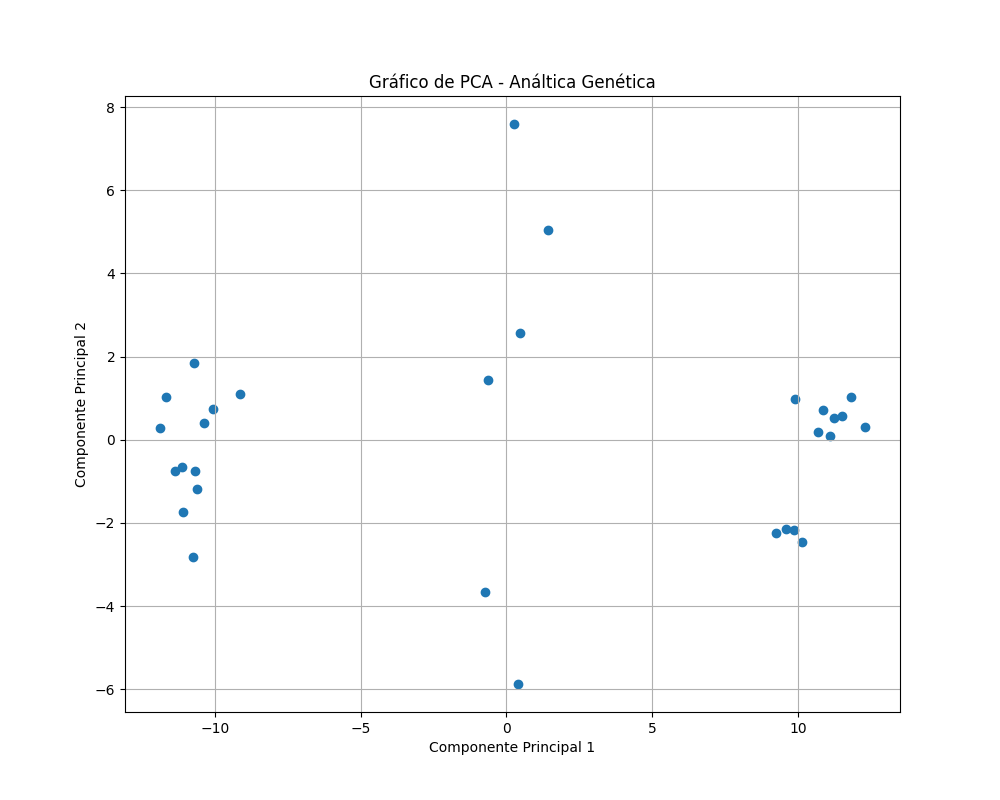
\includegraphics[width=0.85\textwidth]{../resultados/grafico_pca.png}
\caption{Scatter plot de PC1 vs PC2. Cada punto representa un individuo. Se observan tres grupos bien definidos: Cluster A (derecha, PC1 $\approx$ +10), Cluster B (izquierda, PC1 $\approx$ --11), y un grupo intermedio de individuos de mezcla (centro, PC1 $\approx$ 0).}
\label{fig:pca}
\end{figure}

\subsection{Coordenadas Principales}

\begin{table}[H]
\centering
\caption{Coordenadas PC1 y PC2 para los 30 individuos analizados.}
\label{tab:coordenadas}
\footnotesize
\begin{tabular}{@{}lcc|lcc@{}}
\toprule
\textbf{Individuo} & \textbf{PC1} & \textbf{PC2} & \textbf{Individuo} & \textbf{PC1} & \textbf{PC2} \\ \midrule
Individuo\_1  & $+9.890$  & $+0.977$  & Individuo\_16 & $-11.368$ & $-0.758$ \\
Individuo\_2  & $+11.088$ & $+0.084$  & Individuo\_17 & $-10.592$ & $-1.194$ \\
Individuo\_3  & $+11.814$ & $+1.022$  & Individuo\_18 & $-11.669$ & $+1.025$ \\
Individuo\_4  & $+9.873$  & $-2.176$  & Individuo\_19 & $-11.105$ & $-1.729$ \\
Individuo\_5  & $+9.245$  & $-2.245$  & Individuo\_20 & $-10.069$ & $+0.734$ \\
Individuo\_6  & $+10.861$ & $+0.722$  & Individuo\_21 & $-10.752$ & $-2.820$ \\
Individuo\_7  & $+11.252$ & $+0.519$  & Individuo\_22 & $-10.707$ & $+1.843$ \\
Individuo\_8  & $+9.602$  & $-2.137$  & Individuo\_23 & $-11.123$ & $-0.646$ \\
Individuo\_9  & $+10.678$ & $+0.182$  & Individuo\_24 & $-10.361$ & $+0.408$ \\
Individuo\_10 & $+11.522$ & $+0.571$  & Individuo\_25 & $+1.417$  & $+5.039$ \\
Individuo\_11 & $+10.133$ & $-2.449$  & Individuo\_26 & $-0.633$  & $+1.449$ \\
Individuo\_12 & $+12.292$ & $+0.308$  & Individuo\_27 & $+0.454$  & $+2.573$ \\
Individuo\_13 & $-11.870$ & $+0.289$  & Individuo\_28 & $-0.743$  & $-3.668$ \\
Individuo\_14 & $-10.668$ & $-0.755$  & Individuo\_29 & $+0.403$  & $-5.872$ \\
Individuo\_15 & $-9.130$  & $+1.112$  & Individuo\_30 & $+0.269$  & $+7.592$ \\ \bottomrule
\end{tabular}
\end{table}

% ---------- 5. ANALISIS COMPARATIVO ----------
\section{An\'{a}lisis de Estructura Poblacional}\label{sec:analisis}

\subsection{Identificaci\'{o}n de Clusters}

Los resultados obtenidos revelan una estructura poblacional tripartita claramente definida:

\begin{enumerate}
    \item \textbf{Cluster A --- Poblaci\'{o}n de referencia 1 (Individuos 1--12):} Ubicados en el semiplano derecho con PC1 $\approx +10$ y PC2 disperso alrededor de 0. Este grupo muestra alta cohesi\'{o}n interna, con desviaciones est\'{a}ndar de PC1 y PC2 de $0.89$ y $1.15$ respectivamente. La homogeneidad gen\'{e}tica de la poblacion sugiere una poblaci\'{o}n con historia reproductiva aislada.

    \item \textbf{Cluster B --- Poblaci\'{o}n de referencia 2 (Individuos 13--24):} Ubicados en el semiplano izquierdo con PC1 $\approx -11$ y PC2 disperso alrededor de 0. Similarmente cohesivo, con desviaciones est\'{a}ndar de $0.73$ (PC1) y $1.16$ (PC2). La separaci\'{o}n casi sim\'{e}trica respecto al origen en PC1 indica una divergencia gen\'{e}tica equilibrada entre ambas poblaciones.

    \item \textbf{Grupo Intermedio --- Individuos de mezcla (Individuos 25--30):} Posicionados en la zona central del gr\'{a}fico (PC1 $\approx 0$), con PC2 mostrando alta dispersi\'{o}n vertical ($\sigma_{\text{PC2}} = 4.78$). Esta configuraci\'{o}n es el sello distintivo que define \emph{admixture} o mezcla gen\'{e}tica.
\end{enumerate}

\subsection{An\'{a}lisis de Mezcla (Admixture)}

La posici\'{o}n intermedia de los Individuos 25--30 en el eje PC1 es evidencia directa de ancestros compartidos entre las Poblaciones A y B. En t\'{e}rminos de su historia gen\'{e}tica, estos individuos son descendientes de eventos de hibridaci\'{o}n o migraci\'{o}n entre las dos poblaciones parentales.

El patr\'{o}n observado se interpreta como sigue:

\begin{itemize}
    \item \textbf{PC1 como eje de divergencia poblacional:} Captura la direcci\'{o}n de m\'{a}xima varianza gen\'{e}tica, que en este caso separa las dos poblaciones parentales. Los individuos de mezcla tienen PC1 $\approx 0$ porque heredan aproximadamente la misma proporci\'{o}n de alelos de ambas poblaciones.
    
    \item \textbf{PC2 como eje de variaci\'{o}n secundaria:} La alta dispersi\'{o}n en PC2 de los individuos intermedios refleja la variabilidad en la proporci\'{o}n exacta de mezcla. Por ejemplo, el Individuo\_30 (PC2 = +7.59) y el Individuo\_29 (PC2 = --5.87) representan extremos dentro del espectro de mezcla, posiblemente con diferentes proporciones de ancestros A y B.
    

\subsection{Verificaci\'{o}n de la Normalizaci\'{o}n de Patterson}

El test de verificaci\'{o}n confirm\'{o} que la media de cada columna de $\tilde{G}$ es $\|\text{media}\|_\infty < 10^{-10}$, validando que la normalizaci\'{o}n de Patterson produce z-scores gen\'{e}ticos centrados. La varianza por columna se aproxima a 1, consistente con el modelo Wright-Fisher neutro.

\end{itemize}

% ---------- 6. CONCLUSIONES ----------
\section{Conclusiones}\label{sec:conclusiones}

\begin{enumerate}
    \item Se implement\'{o} exitosamente un pipeline completo de PCA gen\'{e}tico en C++17, desde la carga de datos genot\'{i}picos hasta la proyecci\'{o}n y visualizaci\'{o}n de componentes principales, con arquitectura modular documentada bajo metodolog\'{i}a SSD.

    \item La normalizaci\'{o}n de Patterson garantiz\'{o} que cada SNP contribuyera equitativamente al an\'{a}lisis, evitando el sesgo por frecuencias al\'{e}licas extremas y validando la hip\'{o}tesis de deriva gen\'{e}tica neutra.

    \item El algoritmo \texttt{BDCSVD} de Eigen demostr\'{o} ser num\'{e}ricamente estable, convergiendo sin excepciones y produciendo una factorizaci\'{o}n ortogonal con precisi\'{o}n de m\'{a}quina.

    \item Los resultados revelan una estructura poblacional tripartita: dos poblaciones parentales bien diferenciadas (Clusters A y B) y un grupo de 6 individuos intermedios que evidencian procesos de mezcla gen\'{e}tica (admixture), consistentes con eventos hist\'{o}ricos de migraci\'{o}n o hibridaci\'{o}n.

    \item PC1 captura el $57.11\%$ de la varianza gen\'{e}tica total y constituye el eje principal de divergencia poblacional, mientras que PC2 ($3.77\%$) captura la variaci\'{o}n secundaria, incluyendo la dispersi\'{o}n dentro del grupo de mezcla.
\end{enumerate}

% ---------- REFERENCIAS ----------
\begin{thebibliography}{9}
\bibitem{patterson2006} Patterson, N., Price, A. L., \& Reich, D. (2006). Population structure and eigenanalysis. \textit{PLoS Genetics}, 2(12), e190.

\bibitem{price2006} Price, A. L., et al. (2006). Principal components analysis corrects for stratification in genome-wide association studies. \textit{Nature Genetics}, 38(8), 904--909.

\bibitem{trefethen1997} Trefethen, L. N., \& Bau III, D. (1997). \textit{Numerical Linear Algebra}. SIAM.

\bibitem{golub2013} Golub, G. H., \& Van Loan, C. F. (2013). \textit{Matrix Computations} (4th ed.). Johns Hopkins University Press.

\bibitem{eigen} Eigen Documentation. \textit{SVD Module.} \url{https://eigen.tuxfamily.org/dox/group__SVD__Module.html}
\end{thebibliography}

\end{document}